%----------------------------------------------------------------------------------------
%	PACKAGES AND DOCUMENT CONFIGURATIONS
%----------------------------------------------------------------------------------------

\documentclass[a4paper,12pt]{article}
\usepackage{geometry}
\usepackage{appendix}
\usepackage{amsfonts,amsmath,amssymb}
\usepackage{enumerate}
\usepackage{float}
\usepackage{geometry}
\usepackage{bookmark}
\usepackage{latexsym}
\usepackage{listings}
\usepackage{multicol,multirow,multido}
\usepackage{siunitx} % Provides the \SI{}{} and \si{} command for typesetting SI units
\usepackage{graphicx} % Required for the inclusion of images
\usepackage{subfigure}
\usepackage{graphicx} % Required for the inclusion of images
\usepackage{subfigure}
\usepackage{multirow}
\usepackage{amsmath} % Required for some math elements 
\usepackage{indentfirst}
\usepackage{times} % Uncomment to use the Times New Roman font
\usepackage{cite}
\usepackage{appendix}
\usepackage{verbatim}
\usepackage{draftwatermark}
\SetWatermarkText{Dzsyang}
\SetWatermarkLightness{0.95}
\SetWatermarkScale{0.4}  
\usepackage[T1]{fontenc}
\usepackage{lastpage}
\usepackage{tabularx}
\usepackage{booktabs}
\usepackage[labelfont=bf,format=plain,justification=centering,singlelinecheck=false]{caption}
\usepackage{fancyhdr} 
\usepackage{makecell}
\hypersetup{
colorlinks=true,
linkcolor=black
}
\pagestyle{fancy}
\fancyhf{}
\rhead{page \thepage\ of \pageref{LastPage}}
\lhead{VC210 Dzsyang}
%\usepackage{float}

%----------------------------------------------------------------------------------------
%	DOCUMENT INFORMATION
%----------------------------------------------------------------------------------------
\begin{document}

\title{\huge VC210 Notes} 
\author{Dzsyang}
\date{November 14, 2022}

\maketitle % Insert the title, author and date
\thispagestyle{fancy}

\begin{center}

\large Fall 2022\par
\large Prof. Milias Liu\par
\large UM-SJTU Joint Institute
\end{center}

\newpage

\tableofcontents

\newpage



\newpage
%----------------------------------------------------------------------------------------
%	Section 1
%----------------------------------------------------------------------------------------
\section{Foundamentals}
\subsection{Chemistry at Three Levels}
\textbf{Macroscopic} level: dealing with the properties of large, visible objects.\par
\textbf{Microscopic} level: dealing with the rearrangements of atoms.\par
\textbf{Symbolic} level: using terms, chemical symbols, and mathematical equations.\par
A chemist thinks at the microscopic level, conducts experiments at the macroscopic level, and represents both symbolically.
\subsection{Nuclear Model}
$p^{+} = 1.673\times10^{-27} kg, n^{0} = 1.675\times10^{-27} kg$.\par $p^{+}$ and $n^{0}$ are 2000 times heavier than an $e^{-}$.\par
\textbf{Isotopes} of an element have the same atomic number but different mass numbers. Their nuclei have the same number of protons but different numbers of neutrons. The chemical properties of all the atom’s isotopes are the same.
\subsection{Properties}
\textbf{Extensive properties}: Volume, Mass;  
\textbf{Intensive properties}: Density, Temperature
\subsection{Energy}
\textbf{Kinetic} is the energy that a body possesses due to motion.\par
\textbf{Potential} is the energy that a body possesses due to its position in a field of force.\par
\textbf{Electromagnetic} is the energy due to attractions and repulsions between electric charges.
\subsection{Mixtures}
\textbf{Heterogeneous}: components are visible with a microscope or an unaided eye. (Milk)\par
\textbf{Homogeneous}: well mixed into a single phase; a microscope cannot distinguish the particles. (Sugar water)
\subsection{Separation}
\begin{center}
  \begin{tabular}{cc}
    \toprule
    Distillation    & Boiling Points  \\
    Chromatography  & Absorption ability  \\
    Decanting  & Density \\
    Filtration  & Particle size and solubility  \\
    \bottomrule
  \end{tabular}
\end{center}







\newpage
%----------------------------------------------------------------------------------------
%	Section 2
%----------------------------------------------------------------------------------------
\section{Atomic Theory}

\newpage
%----------------------------------------------------------------------------------------
%	Section 3
%----------------------------------------------------------------------------------------
\section{Basic Quantum Mechanics}

\newpage
%----------------------------------------------------------------------------------------
%	Section 4
%----------------------------------------------------------------------------------------
\section{Molecular Shapes, VSEPR, VB and MO Theory}

\newpage
%----------------------------------------------------------------------------------------
%	Section 5
%----------------------------------------------------------------------------------------
\section{Chemical Bonds}

\newpage
%----------------------------------------------------------------------------------------
%	Section 6
%----------------------------------------------------------------------------------------
\section{Gases}
\subsection{The Nature of Gases} Eleven elements are gases under normal conditions: H, He, N, O, F, Ne, Cl, Ar, Kr, Xe, Rn. Low molar mass compounds such as carbon dioxide, hydrogen chlorideare also gases.
\subsection{The Unit of Pressure}
$1 Pa=1 kg\cdot m^{-1}\cdot s^{-2}$. $10^{5} Pa=1 bar$.\par $760 mmHg=760 Torr=1atm=1.013\times 10^{5} Pa$.
\subsection{The Gas Laws}
\textbf{Boyle's Pressure Experiment} $PV=Const.$\par
\textbf{Charles' Law} $V/T=Const.$\par No real gas has zero volume. Lowest possible temperature: -273.15°C.
\subsection{Avogadro's Principle}
All gases occupy the same volume under the same conditions of temperature
and pressures. The molar volume of all gases is close to $22.4 L\cdot mol^{-1}$ at 0 °C and 1 atm.
\subsection{Standard Conditions}
\noindent\textbf{Standard Ambient Temperature and Pressure (SATP)}\par SATP means exactly 25 °C (298.15 K) and exactly 1 bar. The molar volume of an ideal gas is $24.79 L\cdot mol^{-1}$.\\
\noindent\textbf{Standard Temperature and Pressure (STP)}\par STP means 0 °C (273.15 K) and 1 atm (both exactly).
The molar volume of an ideal gas is $22.41 L\cdot mol^{-1}$.
\subsection{The Ideal Gas Law}
\begin{center}
$pV=nRT$
\end{center}\par
The constant $R = 8.314 J\cdot K^{-1}\cdot mol^{-1}$.\par
The ideal gas law is a limiting law, valid only as $p\rightarrow0$.\par
The differences between idel gases and real gases are significant at high pressures and low temperatures.
\subsection{Combined Gas Law}
\begin{center}
$\dfrac{p_{1}V_{1}}{n_{1}T_{1}}=\dfrac{p_{2}V_{2}}{n_{2}T_{2}}$
\end{center}
\subsection{Change n for The Ideal Gas Law}
\textbf{Molar Concentration} $M=\dfrac{p}{RT}$.\par
\textbf{Gas Density} $d=\dfrac{Mp}{RT}$.
\subsection{Mixtures of Gases}
A mixture of gases behaves like a single pure gas.\par
\textbf{Dalton's Law of Partial Pressures}\par
Dalton concluded that the total pressure is the sum of the individual pressures of each gas.
\begin{center}
$\chi_{A}=\dfrac{n_{A}}{n_{A}+n_{B}+...}$, $p_{A}=\chi_{A}p_{T}$
\end{center}
\subsection{The Kinetic Model of Gases}
The kinetic model (KMT) of a gas allows us to derive the quantitative relation between pressure and the speeds of the molecules.\par
\textbf{Root Mean Square Speed} $v_{rms}=\sqrt\frac{3RT}{M}$.\par
\textbf{Most Possible Speed} $v_{rms}=\sqrt\frac{2RT}{M}$.\par
\textbf{Effusion} In effusion, molecules escape through a small hole in a barrier into a region of low pressure. And we can find $\overline{v}\propto \frac{1}{\sqrt{m}}$.\par
\textbf{The Maxwell Distribution of Speeds} $f(v)=4\pi (\frac{M}{2\pi RT})^{\frac{3}{2}}v^{2}e^{-Mv^{2}/2RT}$.\par
For the same temparature, the greater the molar mass, the lower the speed.\par
For the same molar mass, the higher the temperature, the higher the average speed and the broader the spread of speeds.
\subsection{Deviations from Ideality}
Gases can be condensed to liquids when cooled or compressed.\par
A measurement of the compression factor $Z=\frac{V_{m, real}}{V_{m, ideal}}$.\par
At low pressures the attractive forces are dominant and $Z<1$.\par
At high pressures, repulsive forces become dominant and $Z>1$ for all gases.\par
\subsection{van der Waals Equation} 
$(p+a\frac{n^{2}}{V^{2}})(V-nb)=nRT$.\par
Parameter "a" represents the attraction between molecules; the value is large for strongly attracting molecules.
Parameter "b" represents the role of repulsions; it can be thought of as representing the volume.

\newpage
%----------------------------------------------------------------------------------------
%	Section 7
%----------------------------------------------------------------------------------------
\section{Liquids and Solids}
\subsection{Different Types of Intermolecular Forces}
\begin{center}
  \begin{tabular}{ccc}
    \toprule
    Type of interaction & $E_{p}$ dependence & Interacting species \\
    \hline
    ion-ion    & $1/r$  & ions  \\
    ion-dipole  & $1/r^{2}$  & ions and polar molecules  \\
    dipole-dipole (stationary)  & $1/r^{3}$  & stationary polar molecules  \\
    dipole-dipole (rotating)  & $1/r^{6}$  &rotating polar molecules  \\
    hydrogen bonding &   &special case of dipole-dipole: N-H, O-H, F-H  \\
    \bottomrule
  \end{tabular}
\end{center}
\subsection{London Forces}
Attractive forces between nonpolar molecules are London forces.\par
Even nonpolar noble gases can be liquefied, as well as many nonpolar compounds.\par
\textbf{London interaction} $E_{p} \propto \dfrac{\alpha_{1}\alpha_{2}}{r^{6}}$.\par
\textbf{Influence}\par
Size: As size increases (more shells) $\Rightarrow$ polarizability increases $\Rightarrow$ melting and boiling points increase.\par
Shape: Rod-like molecules have a greater surface area, more contact points for molecules to join together (high melting and boiling points); Ball or spherical shaped molecules have fewer contact points for molecules to join together (low melting and boiling points).
\subsection{Hydrogen Bonding}
Very strong interaction between molecules that is specific to molecules with certain types of atoms (the second strongest only to ion-ion interaction).\par
A hydrogen bond is denoted by a dotted line, $X-H...X$, X = N, O, F.
\subsection{Surface Tension}
\textbf{Viscosity} is a liquid’s resistance to flow: the higher the viscosity of the liquid,
the more sluggish the flow. ↑Viscosity indicates, ↑intermolecular strength.\par
\textbf{Surface tension} is the reason that the surface of a liquid is smooth. Strong forces pull the molecules together, with a net inward pull.\par
The upward curved meniscus (concave) of water forms because both water and glass have comparable forces: Adhesion $\approx$ Cohesion.\par
The downward meniscus (convex) of mercury forms because the cohesive forces in mercury is stronger than between mercury atoms and the glass: Cohesion $>$ Adhesion.
\subsection{Liquid Crystals}
Liquid crystals are neither a solid nor a liquid, but an intermediate called a mesophase. Here molecules have the fluidity of a liquid and some of the order of a molecular solid. They are responsive to changes in temperature and electric fields.\par
Anisotropic materials depend on the direction of measurement. Isotropic materials do not depend on orientation: water’s viscosity is the same in all directions.\par
\textbf{Three phases}\par
Nematic phase: parallel molecules, staggered along their long axes.\par
Smectic phase: molecules are parallel and line up to form sheets.\par
Cholesteric phase: sheets of parallel molecules are rotated relative to their neighbors and form a helical structure.\par
\textbf{LCD (liquid-crystal display)} Light is polarized when a potential difference is applied. The molecules rotate until they are oriented with the electric field and become opaque, forming dark spots on a screen.
\subsection{Solids Types}
\textbf{Crystalline and Amorphous Solids} Crystalline solids have long-range order. Amorphous solids have short-range order.\par
\textbf{Molecular Solids} Molecular solids are held together by intermolecular forces.\par
\textbf{Network Solids} Atoms in network solids are joined to their neighbors by strong covalent bonds. Therefore, network solids are very hard, rigid materials with high melting and boiling points.\par
\textbf{Metallic Solids} Metals are cations bound tightly together by a sea of swirling electrons that the metals have lost. Many metallic structures are closed-packed (layer upon layer).\par
\textbf{Closed-packed Structures} ABABAB pattern: Hexagonal closed-pack (hcp); ABCABC pattern: Cubic closed-pack (ccp).
\subsection{Unit Cells}
The smallest region of the crystal lattice that repeats itself is referred to as the unit cell. The atoms in a unit cell can stack,
or arrange themselves, into one of three types of cubic structures: 1. Primitive cubic; 2. Body-centered cubic; 3. Cubic closed-packed.\par
\noindent(4. Face-centered close packed; 5. Hexagonal close packed)
\begin{figure}[b]
\centering
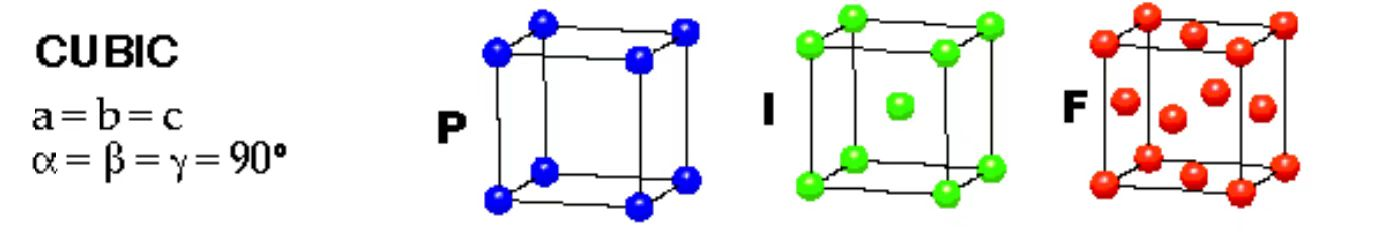
\includegraphics[width=9.5cm,height=1.5cm]{unitcell.png}
\end{figure}


\newpage
%----------------------------------------------------------------------------------------
%	Section 8
%----------------------------------------------------------------------------------------
\section{The First Law of Thermodynamics}
\subsection{Historical Views on Heat}
\textbf{Sadi Carnot} Heat flowed to produce work.\par
\textbf{James Joule} Energy can be transformed into heat and/or work.\par
\subsection{System versus Surroundings}
The system and the surroundings jointly make up the universe.\par
System to the surroundings: Open, Close, Isolate:\par
Open: Exchange both matter and energy;\par
Close: Exchange energy;\par
Isolate: No contact.
\subsection{Formula}
$\Delta U = Q + W$. i.e., $Q=\Delta U+p\Delta V$.
\subsection{Internal Energy U}
In thermodynamics, the capacity of a system to do work is called its internal energy U. Absolute internal energy is not measurable because it includes the energies of all the atoms, their electrons, and the components of their nuclei.\par
Internal energy is energy stored in a system as kinetic energy and potential energy.\par
The internal energy of an isolated system is constant.
\subsection{Work}
\textbf{Expansion work} is a change in volume of a system. $W=-p\Delta V$.\par
Two forms:\par Isobar (Constant pressure);\par Isothermal (Constant temperature) $W=-nRTln\frac{V_{final}}{V_{initial}}$.\par
Expansion against zero pressure is called free expansion.\par
\textbf{Nonexpansion work} can be the flow of electrical current.
\subsection{Heat Capacity}
Specific heat capacity: $Q = m C_{s} \Delta T$ (for water $4.18 J\cdot K^{-1}\cdot g^{-1}$);\par
Molar heat capacity: $Q = n C_{m} \Delta T$ (for water $75 J\cdot K^{-1}\cdot mol^{-1}$).
\subsection{State Functions}
A property that depends only on the current state of the system and is independent of how that state was prepared is called a state function.\par
Such as pressure, volume, temperature, mass, altitude and internal energy.
\subsection{The Origin of Internal Energy}
The \textbf{equipartition theorem} (not derived here) states the average value of each quadratic contribution at a temperature $T$ is equal to $\frac{1}{2}kT$.\par
For monoatomic molecules: Total $E_{kin}$: $\frac{3}{2}RT = 3.72 kJ\cdot mol^{-1}$;\par
For linear molecules: Total $E_{kin}$: $\frac{5}{2}RT = 6.02 kJ\cdot mol^{-1}$;\par
For nonlinear molecules: Total $E_{kin}$: $\frac{6}{2}RT = 7.44 kJ\cdot mol^{-1}$.
\subsection{Enthalpy}
$H = U + pV$. i.e., $\Delta H =\Delta U + p\Delta V=Q+(p-p_{ex})\Delta V$.\par
For a chemical reaction open to the atmosphere, or at constant pressure, the heat released or required is the enthalpy of the system. $\Delta H=Q$. Therefore, $\Delta H<0$ for exothermic reactions, "-"; $\Delta H>0$ for endothermic reactions, "+".\par
\textbf{Vaporisation} $\Delta H_{vap,m} = H_{m}(vapor) - H_{m}(liquid)$, where $\Delta H_{m}$ is the molar heat.\par
\textbf{Fusion} $\Delta H_{fus,m} = H_{m}(liquid) - H_{m}(solid)$.\par
\textbf{Freezing} $\Delta H_{fre,m} =-\Delta H_{vap,m}$. \textbf{Condensation} $\Delta H_{con,m} =-\Delta H_{fus,m}$.\par
\textbf{Sublimation}  $\Delta H_{sub,m} = H_{m}(vapor) - H_{m}(solid)$. \textbf{Deposition}  $\Delta H_{dep,m} = -\Delta H_{sub,m}$.
\subsection{The Relation between H and U}
At constant volume, the heat transfer is $\Delta U$; $C_{V,m}=\frac{ \Delta U}{\Delta T}$.\par
At constant pressure, it is $\Delta H$; $C_{p,m} = C_{V,m} + R$.\par
\subsection{Hess’s Law}
The overall reaction enthalpy is the sum of the reaction enthalpies of each step.
\subsection{The Born-Haber Cycle}
In a Born-Haber cycle, we\par
a) break apart the bulk elements into atoms,\par
b) ionize the atoms,\par
c) combine the gaseous ions to form the ionic solid,\par
d) then form the elements again from the ionic solid.

\newpage
%----------------------------------------------------------------------------------------
%	Section 9
%----------------------------------------------------------------------------------------
\section{The Second and Third Laws of Thermodynamics}
\subsection{Entropy and Disorder}
Entropy, $S$, is a measure of disorder.\par
Low entropy means little disorder.
High entropy means great disorder.\par
In an isolated system the entropy increases in the course of any spontaneous change.\par
The natural progression of a system and its surroundings is from order to disorder, from lower to higher entropy.\par
An entropy change in a system is calculated as: $\Delta S = \dfrac{q_{rev}}{T}$.\par
Entropy can predict the natural direction of a reaction.
\subsection{Deriving a Change in Entropy}
Changes in temperature: $\Delta S=Cln\dfrac{T_{2}}{T_{1}}$.\par
Changes in volume: $\Delta S=nRln\dfrac{V_{2}}{V_{1}}$.\par
Changes in pressure: $\Delta S=nRln\dfrac{p_{1}}{p_{2}}$.
\subsection{A Molecular Interpretation of Entropy}
The entropies of all perfect crystals approach zero as the absolute temperature approaches zero.\par
The entropy of any substance to be greater than zero above $T = 0$.
\subsection{Boltzmann Formula - Statistical Entropy}
$S=klnW$, where $k = 1.381 \times 10^{-23} J\cdot K^{-1}$, $W$ is the number of positions atoms or molecules can arrange into and are called microstates.\par
$W=\Pi$ orientations of each molecule.
\subsection{Standard Molar Entropies}
$\Delta S^{\circ}=\dfrac{\Delta H^{\circ}}{T}$.\par
Complex molecules have greater entropy values. Heavier molecules have greater entropy values.
\subsection{Global Changes in Entropy: Total}
$\Delta S(total)=\Delta S (system)-\Delta S(surroundings)$.\par
$\Delta S(system)=\Sigma nS_{m}(products)-\Sigma nS_{m}(reactants)$.\par
$\Delta S(surroundings)=-\dfrac{\Delta H}{T}$.\par
If $\Delta S(total)$ is positive (an increase), the process is spontaneous.\par
If $\Delta S(total)$ is negative (a decrease), the reverse process is spontaneous.\par
If $\Delta S(total) = 0$, the process has no tendency to proceed in either direction (phase changes are the most common examples of when $\Delta S(total) = 0$).\par
\textbf{Clausius inequality} In an isolated system $q=0$ so $\Delta S\geq0$, meaning the entropy cannot decrease in an isolated system, or in other words, the entropy of the universe is steadily increasing.
\subsection{Equilibrium}
A system at equilibrium has no tendency to change in either direction (forward or reverse).
The equilibrium state is a dynamic equilibrium, where the forward and reverse processes are continually at matching rates.
\subsection{Gibbs Free Energy}
Gibbs free energy accomplishes the same task more simply, and it also tells us how much nonexpansion work (work under free expansion when $W$ usually = 0) we can get from the system.\par
Gibbs free energy is a measure of the energy free to do nonexpansion work.\par
$G = H - TS$. i.e., $\Delta G =\Delta H - T\Delta S$.\par
When $\Delta G$ is large "-" the process is spontaneous.\par
\textbf{Labile versus inert}\par
If $\Delta G_{f}^{\circ}<0$, then elements are poised to change spontaneously into the compound.\par
If $\Delta G_{f}^{\circ}>0$, then the compound is poised to change spontaneously into the pure elements (unstable).\par
\textbf{The crossover point} is where $\Delta G_{f}^{\circ}$ goes from "+" to "-".\par Therefore, we can take $\Delta G^{\circ}$ = $\Delta H^{\circ}$ – T$\Delta S^{\circ}$ set it to 0, i.e., $T=\dfrac{\Delta H^{\circ}}{\Delta S^{\circ}}$.

\newpage
%----------------------------------------------------------------------------------------
%	Section 10
%----------------------------------------------------------------------------------------
\section{Physical Equilibrium}
\subsection{Phases and Phase Transitions}
Matter exists in a single phase such as a solid, liquid, or gas. A phase change occurs when converting one phase into another.\par
Carbon has three distinct solid phases: diamond, graphite, and Buckminster fullerenes (C60). Helium is only known to exist as a gas and liquid.
\subsection{Vapour Pressure}
Evapouration takes place at the surface because molecules are bound to fewer neighbors.A dynamic equilibrium is when the rate of escaping matches the rate of returning.\par
Solids and gases aside, liquids with weak intermolecular forces have the highest vapour pressure; Liquids with strong intermolecular forces, ones capable of forming hydrogen bonds, have the lowest vapour pressure.
\subsection{Clausius - Clapeyron Equation}
$ln\dfrac{p_{2}}{p_{1}}=\dfrac{\Delta H_{vap}^{\circ}}{R}(\dfrac{1}{T_{1}}-\dfrac{1}{T_{2}})$.
\subsection{Water is Unusual}
Most substances are more dense in the solid phase than liquid, water being an exception. Water is highly unusual, at 0.0°C,  $density_{liquid} > density_{solid}$.\par
Solid water hydrogen bonds hold the molecules apart at low temperatures. As ice melts, the hydrogen bonds collapse, allowing water molecules to pack more closely.
\subsection{Phase Diagram}
A phase diagram is a map showing phases at different pressures and temperatures.\par
\textbf{For water}, a triple point is the temperature and pressure at which water exists as a solid, liquid, and vapour. The slope of the solid–liquid boundary depends on the relative density and for liquid water it is more dense than its solid.\par
\textbf{Critical Properties} \par
There is an end in the liquid–vapour phase boundary called the critical point. \par
The density of the vapour is so great that it is equal to the density of the liquid.\par
 The surface boundary disappears into a single, uniform phase.\par
Here, the critical pressure and critical temperature mark the end of either liquid or vapour, and is now a supercritical fluid, a very dense fluid.
\subsection{Raoult's Law}
$p=\chi_{solvent}\cdot p_{pure}$, where $p$ is the vapour pressure of the solvent, $\chi_{solvent}$ is the mole fraction of the solvent, and $p_{pure}$ is the vapour pressure of the pure solvent.\par
$\chi_{solvent} =\dfrac{n_{solvent}}{n_{solute} + n_{solvent}}$.\par
$\chi_{A,vapour} =\dfrac{\chi_{A,liquid}\cdot p_{A,pure}} {{\chi_{A,liquid\cdot} p_{A,pure} + \chi_{B,liquid}\cdot p_{B,pure}}}$.
\subsection{Distillation}
The vapour pressure as well as the boiling point of the mixture will be intermediate between the two pure liquids.\par
\textbf{Fractional distillation} is a continuous re-distillation. \par
Higher BP (Boiling Point) vapour condenses and vapourizes over and over as it rises; the lower BP liquid drips back into the boiling mixture.
Vapour becomes richer in the component with the lower boiling point. The final distillate is nearly pure (lower BP liquid), and the liquid in the pot is also nearly pure (higher BP liquid).
\subsection{Pressure and Gas Solubility: Henry's Law}
The solubility of a gas is directly proportional to its partial pressure: $s = k_{H}p$, where $k_{H}$ is called Henry's constant.
\subsection{Enthalpy of Solution}
Measuring heat released or absorbed when a substance dissolves is called molar enthalpy of solution, $\Delta H_{sol}$.\par
The first step sublimes solid ions to gas ions. Highly endothermic, this is the lattice enthalpy, $\Delta H_{L}$;\par
In the second step, gaseous ions plunge into water forming the final solution. This is the enthalpy of hydration, $\Delta H_{hyd}$;\par
Combining these steps: $\Delta H_{sol}=\Delta H_{L}+\Delta H_{hyd}$.\par
High charge and small ionic radius contribute to high lattice enthalpy ($\Delta H_{L}$). However, often these can be the same properties that relate to low enthalpy of hydration ($\Delta H_{hyd}$). Therefore it is very difficult to make reliable predictions and instead rationalise what is observed.
\subsection{Solubility}
\textbf{Limits}: unsaturated and saturated solution.\par
\textbf{Like Dissolves Like}: polar-polar, nonpolar-nonpolar.
\subsection{Collgative Properties}
Properties that depend on the numbers of solute and solvent molecules and not on chemical identity are called colligative properties.\par
Four colligative properties of major importance are the:\par
1. lowering of the vapour pressure,\par
2. raising boiling points,\par
3. lowering of freezing points, and\par
4. osmosis.\par
Colligative properties are measured using either mole fraction ($\chi_{A}=\dfrac{n_{A}}{n_{A}+n_{B}+...}$) or molality ($\dfrac{n_{solute}(mol)}{m_{solvent}(kg)}$).
\subsection{Boiling-Point Elevation and Freezing-Point Depression}
A nonvolatile solute lowers the vapour pressure of the solvent, therefore increasing the boiling point and therefore it is called boiling-point elevation. The increased boiling temperature is usually quite small and is of little practical importance in science.\par
Freezing-point depression is more significant. An added solute lowers of the freezing point of a solvent. Melting point are also a method for determining the purity of a solid.\par
Boiling-point elevation = $k_{b}$ × molality, temperature increases.\par
Freezing-point depression = $k_{f}$ × molality, temperature decreases.
\subsection{Van't Hoff i Factor}
The van't Hoff $i$ factor, is determined experimentally.\par
In very dilute solution, where all ions are independent, $i$ = number of ions.
\subsection{Osmosis}
\textbf{Osmotic pressure}, $\Pi = iRTc$, where $c$ is molarity.\par
Osmometry is the technique used to determine the molar mass of a solute from osmotic pressure measurements.


\newpage
%----------------------------------------------------------------------------------------
%	Section 11
%----------------------------------------------------------------------------------------
\section{Chemical Equilibrium}
\subsection{Reactions at Equilibrium}
\textbf{The criteria for dynamic chemical equilibrium are:}\par
1. The forward and reverse reactions are both taking place.\par
2. The forward rate equals the reverse rate.\par
Note, it’s impossible to make more product when at equilibrium. The reaction just appears to have stopped moving.
\subsection{Equilibrium Constant K}
$K$ is the same regardless of initial compositions.\par
\textbf{The law of mass action}\par
\begin{center}
$K =(\dfrac{partial\ pressure \ of\ Products}{partial\ pressure\ of\ Reactants})_{equilbrium}$.
\end{center}\par
In general for $a\ A(g) + b\ B(g)\rightleftharpoons  c\ C(g) + d\ D(g)$
\begin{center}
$K_{p} =\dfrac{(p_{C})^{c}(p_{D})^{d}}{(p_{A})^{a}(p_{B})^{b}}$
\end{center}\par
here $p$ means partial pressure, since the reactants and products are gases.\par
It can be shown empirically or thermodynamically that pure liquids or solids do not appear in $K$.\par
\textbf{Aqueous solutions}\par
In general for $a\ A(aq) + b\ B(aq)\rightleftharpoons  c\ C(aq) + d\ D(aq)$
\begin{center}
$K_{C} =\dfrac{[C]^{c}[D]^{d}}{[A]^{a}[B]^{b}}$
\end{center}\par
Note the change to brackets, [ ], signifying, $c$, or molarity, $mol\cdot L^{-1}$.\par
\textbf{Activity}\par
It is common when deriving equations to simplify expressions without units.
\begin{center}
\renewcommand\arraystretch{1.8}
  \begin{tabular}{ccc}
    \toprule
    Summary & Simplified form & Interpretation \\
    \hline
    Ideal gas    & $a_{J} = \dfrac{p_{J}}{p^{0}}$  & [$p^{0} = 1\ bar\ or\ 1\ atm$]  \\
    Solute in a dilute solution  & $a_{J} =\dfrac{ [J]}{c^{0}}$  & [$c^{0} = 1\ mol\cdot L^{-1}$]  \\
    Pure solid or pure liquid  & $a = 1$  & unchanging throughout the reaction \\
    \bottomrule
  \end{tabular}
\end{center}
\subsection{Origins of K and $\Delta$G}
$\Delta G_{r} = \Delta G^{\circ}_{r} + RT ln\dfrac{(a_{C})^{c}(a_{D})^{d}}{(a_{A})^{a}(a_{B})^{b}}$, here $a$ = activity, either a gas or solute in a solution (molarity); $r$ = the overall reaction.\par
\textbf{Reaction quotient} $Q =\dfrac{(a_{C})^{c}(a_{D})^{d}}{(a_{A})^{a}(a_{B})^{b}}$, then $\Delta G_{r} = \Delta G^{\circ}_{r} + RT lnQ$.\par
 Here $K$ is a constant, it is known. $Q$ is unknown and must be found. $Q$ can be larger or smaller than $K$; again it must be calculated.\par
Once $Q = K$ the reaction is at equilibrium, therefore $\Delta G=0$. This leads to\par
$\Delta G^{\circ}=-RTlnK$. This of course links the thermodynamic tables $\Delta G^{\circ}$ to $K$.\par
\subsection{What Does K Mean?}
1. $K << 1$ favours reactants at equilibrium ($\Delta G^{\circ}$ is very positive);\par
2. When $10^{-3} < K < 10^{3}$ neither products nor reactants are favored;\par when ($-10<\Delta G^{\circ}<10$) then temperature will be a factor;\par
3. $K >> 1$ favours products at equilibrium ($\Delta G^{\circ}$ is very negative).
\subsection{The 5\% rule}
The 5\% rule says we can ignore "$x$" when there is less than 5\% decomposition or ionisation change (the definition of a weak acid).\par
A note of good practice is, once solving for $x$, always plug $x$ back into the original equilibrium table to make sure you’re below 5\% and to get your final values.
\subsection{Le Chatelier's Principle}
\textbf{Concentration}\par
Le Chatelier's principle suggests a good way to ensure that a reaction goes on generating a substance: simply remove products as they are formed.\par
\textbf{Inert Gas}\par
Adding an inert gas does not interfere with the reacting gases, so the reacting gases continue to occupy the same volume, and so their individual molar concentrations and partial pressures remain unchanged despite the presence of an inert gas.\par
\textbf{Temperature}\par
Since $\Delta H$ and $\Delta S$ are independent of range of temperatures,\par $ln\dfrac{K_{2}}{K_{1}}=\dfrac{\Delta H^{\circ}}{R}(\dfrac{1}{T_{1}}-\dfrac{1}{T_{2}})$, here we see $K_{2}$ over $K_{1}$ and no "-" on the right.








\newpage
%----------------------------------------------------------------------------------------
%	Section 12
%----------------------------------------------------------------------------------------
\section{Acid-Base}
\subsection{Definitions}
\textbf{Svante Arrhenius}\par
An acid is a compound that contains hydrogen and reacts with water to form hydrogen ($H^{+}$) ions.\par
A base is a compound that produces hydroxide ions ($OH^{-}$) in water.\par
\textbf{Brønsted–Lowry}\par
An acid is a proton donor, and a base is a proton acceptor.\par
A strong acid is fully deprotonated in solution ($\rightarrow$).\par
A weak acid is only partly deprotonated in solution ($\rightleftharpoons$).\par
A strong base is completely protonated in solution ($\rightarrow$).\par
A weak base is only partially protonated in solution ($\rightleftharpoons$).\par
Acid $\xrightarrow{donates\ H^{+}}$ conjugate base. Base $\xrightarrow{accepts\ H^{+}}$ conjugate acid.\par
\textbf{Brønsted vs Arrhenius}\par
Brønsted acids and bases are more general than the Arrhenius definitions.\par
\textbf{Lewis}\par
An acid is an electron pair acceptor.\par
A base is an electron pair donor.\par
\textbf{Lewis vs Brønsted vs Arrhenius}\par
Lewis theory is more general than Brønsted or Arrhenius acid–base theory.
\subsection{Hydronium Ion}
The $H_{3}O^{+}$ ion is called the hydronium ion. We say that the $H_{2}O$ becomes strongly hydrated in a solution to form $H_{3}O^{+}$.
\subsection{Amphiprotic vs Amphoteric}
\textbf{Amphiprotic}: a substance that can be a proton donor or reciever. ($H_{2}O$)\par
\textbf{Amphoteric}: a substance that can behave as either an acid or a base. ($Al$)\par
\subsection{Autoprotolysis Constant}
For $H_{2}O(l) + H_{2}O(l) \rightleftharpoons H_{3}O^{+}(aq) + OH^{-}(aq)$, $K_{w}=[H_{3}O^{+}][OH^{-}]$.\par
In pure water at 25°C, $K_{w}=[H_{3}O^{+}][OH^{-}]=1.0\times 10^{-14}$. The concentrations of $H_{3}O^{+}$ and $OH^{-}$ are very low, which explains why pure water is such a poor conductor of electricity.\par
Autoprotolysis reaction is endothermic, so $K_{w}$ increases with temperature.
\subsection{The pH Scale}
$pH = -log [H_{3}O^{+}]$, $pOH = -log [OH^{-}]$, $pK_{w} = - log K_{w}$. $pH+pOH=pK_{w}$.\par
Most solutions used in chemistry have a pH ranging from 0 to 14, but values outside this range are possible.\par
\subsection{Acid Strength}
There is no general theory that describes acid strength. We only have general trends to work with and compare. 1.Equilibrium constants, $K_{a}$ and $K_{b}$; 2. Solvent.\par
Two different trends are observed, one for periods, the other for groups.\par
\textbf{Period}: Acid strength is based on bond polarity;\par
\textbf{Group}: Acid strength is based on bond strength. ($HF<HCl<HBr<HI$)\par
There are two ways to compare oxoacids.\par
\textbf{In groups with the same number of oxygen atoms}:\par The greater the electronegativity the greater the acidity; ($HClO > HBrO > HIO$)\par
\textbf{A family of the same element with different numbers of oxygen atoms}:\par The greater the number of oxygen atoms, the stronger the acid.
\subsection{The pH of Salt Solutions}
\renewcommand\arraystretch{1.3}
\begin{center}
Common Cations in Water\par
  \begin{tabular}{ccc}
    \toprule
    Character & Interpretation & Examples \\
    \hline
    Acidic    & Conjugate acids of weak bases &$NH_{4}^{+}$ \\
    & Small, highly charged metal cations & $Fe^{3+}, Al^{3+}, Cu^{2+}$ \\
    \hline
    Neutral  & Group 1 and 2 cations & $Li^{+}, Na^{+}, K^{+}, Mg^{+}, Ca^{+}$\\
    & metal cations with charge +1& $Ag^{+}$ \\
    \hline
    Basic  & None&  \\
    \bottomrule
  \end{tabular}
  \end{center}
\begin{center}
Common Anions in Water\par  
  \begin{tabular}{ccc}
    \toprule
    Character & Interpretation & Examples \\
    \hline
    Acidic    & Very few &$HSO_{4}^{-}, H_{2}PO_{4}^{-}$ \\
    \hline
    Neutral  & Conjugate bases of strong acids &$Cl^{-}, Br^{-}, I^{-}, NO_{3}^{-}, ClO_{4}^{-}$ \\
    \hline
    Basic  & Conjugate bases of weak acids& \thead{$F^{-}, O^{2-}, OH^{-}, S^{2-}, HS^{-}, CN^{-}, CO_{3}^{2-},$\\ $PO_{4}^{3-}, NO_{2}^{-}, CH_{3}CO_{2}^{-},$ other carboxylate ions} \\
    \bottomrule
  \end{tabular}
\end{center}
\subsection{The pH of Polyprotic Acids}
For all polyprotic acids or bases, $K_{a_{1}}$ is always the greatest contributor to the overall pH of the solution — except for $H_{2}SO_{4}$.
Only $H_{2}SO_{4}$ has a large $K_{a_{1}}$ and $K_{a_{2}}$.\par
$pH = \frac{1}{2} (pK_{a_{1}} + pK_{a_{2}})$ as long as initial concentration $[X]_{initial} >> K_{a_{1}}$.
\subsection{Very Dilute Solutions}
\textbf{of Strong Acids and Bases}\par
$K_{w} = [H3O^{+}] ([H3O^{+}] - [HCl]_{initial})$.\par
$K_{w} = [H3O^{+}] ([H3O^{+}] - [NaOH]_{initial})$.\par
\textbf{of Weak Acids}\par
Four unknowns exist for a weak acid $HA$, $A^{-}$, $H3O^{+}$, and $OH^{-}$.\par
Both $K_{w} = [H3O^{+}][OH^{-}]$ and $K_{a} = \dfrac{[H3O^{+}][A^{-}]}{[HA]}$ are used to arrive at the following cubic equation.
$[H3O^{+}]^{3} + K_{a}[H3O^{+}]^{2} - (K_{w} + K_{a}[HA]_{initial}])[H3O^{+}] - K_{a}K_{w} = 0$.









\newpage
\end{document}